\chapter{Componentes}
\section{Introducción}
Por lo general, un proyecto de software está compuesto por diferentes funcionalidades, las cuales al juntarse, proveen lo que deseamos que el software realice. Adicionalmente, esas funcionalidades pueden ser usadas individualmente e incluso en otros proyectos. Cada una de ellas se recoge en lo que llamamos componente. Estos elementos se comportan como una caja negra, ya que realizan su función, pero sin mostrar cómo lo hacen internamente. Esto trae ventajas tanto de seguridad, por el encapsulamiento, como de facilidad de uso por las interfaces que provee o solicita.
Por esta razón, la utilización de componentes es ventajosa para realizar este proyecto de software, ya que se generarán componentes independientes que puedan ser reutilizados en un futuro y además, la dependencia entre ellos será baja ya que se gestionarán entre interfaces.
\section{Diagrama de componentes}
\begin{figure}[H]
	\centering
	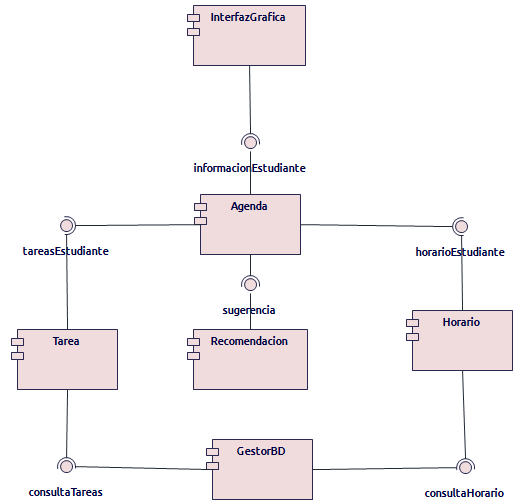
\includegraphics[width=1\linewidth]{diseno/componentes/img/diagramaComponentesv2}
	\caption{Diagrama de componentes}
	\label{fig:componentes}
\end{figure}
Las funcionalidades de los componentes del diagrama son:
\begin{itemize}
	\item Interfaz gráfica: Este componente le ofrece una interfaz gráfica al software, sólo se comunica con el gestorPrincipal para solicitarle la información que necesita mostrar.
	\item Agenda: La agenda organiza las tareas de acuerdo al horario, por lo tanto se comunica con ambos componentes para solicitar la información que necesita para realizar su tarea. Luego le envía la información al componente de interfaz gráfica, para que muestre la información.
	\item Horario: Realiza todas las funciones como crear, modificar, ordenar el horario del estudiante. Se comunica con la persistencia para solicitar información.
	\item Tarea: Se encarga de realizar funciones como crear y  modificar tareas. Se comunica con la persistencia para obtener la información que necesita.
	\item Persistencia: Es el componente que se comunica con la base de datos y brinda fachadas para que los componentes que lo necesiten hagan consultas o ingresen información en la vase de datos.
\end{itemize}
	
